\documentclass[12pt]{article}
\usepackage[utf8]{inputenc}
\usepackage{graphicx}
\usepackage[english, serbian]{babel}
\usepackage[a4paper, top=3cm, bottom=3cm, left=2cm, right=2cm, marginparwidth=1.75cm]{geometry}
\usepackage{newtxtext}
\usepackage{caption}
\captionsetup{justification=centering,singlelinecheck=false}
\captionsetup[table]{position=below,justification=centering,singlelinecheck=false}
\captionsetup[figure]{position=below,justification=centering,singlelinecheck=false}
\usepackage{mathtools}
\usepackage{amssymb}
\usepackage{multicol}
\setlength{\columnsep}{1cm}
\usepackage{lipsum}
\usepackage{listings}
\usepackage[section]{placeins}
\usepackage{subcaption}
\usepackage{fancyhdr}
\usepackage{fancybox}
\usepackage{hyperref}
\usepackage{csquotes}
\usepackage{tikz}
\usetikzlibrary{shapes.geometric, arrows.meta, positioning}
\usepackage[backend=biber, sorting=none]{biblatex}

\addbibresource{ref.bib}

\def\boxx{\mbox{\footnotesize \fbox{${\;\;}^{\!}$}}}
\def\stop{\mbox{\footnotesize {\vrule width 6pt height 6pt}}}

\newcommand*{\addheight}[2][.5ex]{%
  \raisebox{0pt}[\dimexpr\height+(#1)\relax]{#2}%
}

\usepackage[dvipsnames]{xcolor}
\definecolor{deepblue}{rgb}{0,0,0.5}
\definecolor{deepred}{rgb}{0.6,0,0}
\definecolor{deepgreen}{rgb}{0,0.5,0}

\definecolor{codebg}{rgb}{0.96,0.96,0.96}
\lstset{
    backgroundcolor=\color{codebg},
    basicstyle=\ttfamily\footnotesize,
    keywordstyle=\color{deepblue}\bfseries,
    commentstyle=\color{deepgreen},
    stringstyle=\color{deepred},
    breaklines=true,
    numbers=left,
    numberstyle=\tiny\color{gray},
    frame=single,
    captionpos=b,
    showstringspaces=false,
    tabsize=2
}

\renewcommand{\refname}{Literatura}
\renewcommand{\footrulewidth}{1.2pt}
\renewcommand{\headrulewidth}{1.2pt}

\begin{document}

\begin{titlepage}
    \centering

    {\textsc{\Large Univerzitet u Beogradu}}\\[0.5cm]
    {\textsc{\Large Elektrotehnički fakultet}}\\[1.8cm]

    
\includegraphics[width=4.5cm]{slike/etf-logo.jpg}

    \vfill

    {\huge \bfseries \MakeUppercase{Optimalna raspodela poslova na računarima}}\\[0.5cm]
    {\Large Master rad}

    \vfill

    \noindent
    \begin{tabular}{|p{0.47\textwidth}|p{0.47\textwidth}|}
        \hline
        Mentori: & Kandidat: \\ \hline
        dr Jovana Petrović, docent \newline dr Dragan Olćan, profesor & Mihailo Radojević 2023/3209 \\ \hline
    \end{tabular}

    \vspace{2cm}

    {\large Beograd, jul 2026.}\\[0.5cm]

\end{titlepage}


\pagestyle{fancy}
\fancyhead{}
\clearpage

\pagebreak

\section*{Rezime rada}
\addcontentsline{toc}{section}{Rezime rada}

Cilj ovog rada je da se ispita problem maksimizacije zarade pri raspodeli servisa na heterogeni skup računara i da se isti reši primenom genetskog algoritma. U prvom poglavlju formalno je definisan zadatak, izvedena je njegova matematička formulacija kao celobrojni linearni program, navedeni su pristupi rešavanju nelinearnim programiranjem (NLP) i celobrojnim linearnim programiranjem (ILP) sa fokusom na rešavač HiGHS, te su uvedene stohastičke metode kao alternativa za probleme velikih dimenzija. U drugom poglavlju opisana je pretraga rešenja genetskim algoritmom kroz kratku evidenciju koraka algoritma sa pratećim blok dijagramom. U trećem poglavlju prikazani su rezultati za tri instance, problem male dimenzije ($10 \times 10$), problem srednje dimenzije ($100 \times 100$) i problem velike dimenzije ($1000 \times 1000$), uključujući rešenja dobijena rešavačem HiGHS i drugim rešavačima, rešenja genetskog algoritma, poređenje vremena izvršavanja pri istoj hardverskoj konfiguraciji i analizu kumulativnih maksimuma kroz generacije. Četvrto poglavlje sadrži zaključke i pravce daljeg rada.

\pagebreak

\tableofcontents

\pagebreak

\section{Uvod}\label{sec:uvod}

\subsection{Opis problema}

Posmatra se sistem koji se sastoji od $m$ tipova servisa i $n$ heterogenih računara. Svaki servis predstavlja vrstu posla koji treba izvršiti, dok svaki računar predstavlja resurs sa ograničenim radnim vremenom. Za svaki par servis–računar poznato je vreme izvršavanja jedne jedinice servisa na tom računaru i zarada koja se ostvaruje po izvršenoj jedinici. Pored toga, svaki servis ima tržišnu tražnju koja predstavlja maksimalan broj jedinica koje smemo izvršiti u planskom periodu. Svaki računar raspolaže fiksnim radnim vremenom, koje u eksperimentima sprovedenim u ovom radu iznosi $T = 2880$ minuta, što odgovara dva dana.

Zadatak je sledeći. Odrediti koliko jedinica svakog servisa rasporediti na svaki računar tako da ukupna zarada bude maksimalna, a da pritom ne bude prekoračeno ni vreme nijednog računara ni tražnja nijednog servisa. Razlika u vremenima izvršavanja i zaradi po paru servis–računar potiče od činjenice da računari nisu identični. Različite mašine imaju različitu specijalizaciju, pa je profitabilnost izvršavanja istog servisa na različitim mašinama u opštem slučaju različita.

Problem ima jasnu poslovnu interpretaciju. U cloud računarstvu servisi odgovaraju zahtevima korisnika, a računari raznorodnim virtuelnim mašinama. U industrijskoj proizvodnji servisi su artikli koji se izrađuju, a računari su proizvodne linije sa različitim performansama. U logistici servisi predstavljaju tipove paketa, a računari su distributivni centri sa različitim kapacitetima. Bez obzira na konkretni domen primene, matematička struktura problema je ista, što opravdava razvoj generičkih rešavačkih metoda.

Iako je problem konceptualno jednostavan, broj kandidatskih rešenja eksponencijalno raste sa veličinom ulaza. Već za umerene veličine, recimo $100$ servisa i $100$ računara, prostor pretrage prevazilazi mogućnosti naivnih egzaktnih algoritama u prihvatljivom vremenu. Za još veće instance, reda hiljadu servisa i hiljadu računara, komercijalni rešavači mogu pronaći visokokvalitetna rešenja, ali im vreme i memorijski zahtevi značajno rastu. U takvim uslovima stohastičke i metaheurističke metode predstavljaju zanimljivu alternativu, koja žrtvuje garantovanu optimalnost zarad fleksibilnosti i brzog odziva.

\subsection{Matematička formulacija}

Uvedimo sledeće oznake. Neka je $S = \{1, \dots, m\}$ skup servisa, a $C = \{1, \dots, n\}$ skup računara. Neka je $t_{ij}$ vreme izvršavanja jedne jedinice servisa $i \in S$ na računaru $j \in C$, $p_{ij}$ zarada od te jedinice, $d_i$ tražnja za servisom $i$, a $T$ maksimalno radno vreme svakog računara. Promenljive odlučivanja su celobrojne i nenegativne, $x_{ij} \in \mathbb{Z}_{\geq 0}$, gde $x_{ij}$ predstavlja broj jedinica servisa $i$ izvršenih na računaru $j$.

Problem se tada formuliše kao celobrojni linearni program:

\begin{align}
    \max \quad & \sum_{i=1}^{m}\sum_{j=1}^{n} p_{ij} \, x_{ij} \label{eq:obj}\\
    \text{p.o.} \quad & \sum_{i=1}^{m} t_{ij} \, x_{ij} \leq T, \quad \forall j \in C \label{eq:vreme}\\
    & \sum_{j=1}^{n} x_{ij} \leq d_i, \quad \forall i \in S \label{eq:tr}\\
    & x_{ij} \in \mathbb{Z}_{\geq 0}, \quad \forall i \in S, j \in C \label{eq:int}
\end{align}

Funkcija cilja \eqref{eq:obj} predstavlja ukupnu zaradu sumiranu kroz sve servise i sve računare. Ograničenje \eqref{eq:vreme} izražava da ukupno vreme provedeno na računaru $j$ ne sme premašiti $T$. Ograničenje \eqref{eq:tr} izražava da ukupan broj izvršenih jedinica servisa $i$ na svim računarima ne sme premašiti tražnju $d_i$. Uslov celobrojnosti \eqref{eq:int} čini problem računski znatno težim od njegove kontinualne relaksacije.

\subsection{Složenost problema i prostor pretrage}

Razmatrani problem može se posmatrati kao generalizacija problema ranca \cite{MartelloToth1990}. Već za slučaj sa jednim računarom, problem se svodi na ograničeni problem ranca sa više predmeta, što je dobro poznat NP-težak problem. U opštem slučaju, problem se može posmatrati kao varijanta generalizovanog problema dodeljivanja \cite{FisherJaikumar1981, ChuBeasley1997} sa celobrojnim količinama umesto binarnih dodela. Direktna posledica složenosti je da egzaktni rešavači imaju eksponencijalnu vremensku složenost u najgorem slučaju, što motiviše upotrebu stohastičkih i metaheurističkih metoda za velike instance.

Veličina prostora pretrage, ako se zanemare ograničenja, iznosi $\prod_{i,j} (1 + \min(d_i, \lfloor T/t_{ij} \rfloor))$, što za instancu $1000 \times 1000$ daje broj kandidatskih konfiguracija reda veličine $10^{2000}$. Iscrpna pretraga je očigledno neostvariva. Pored eksponencijalnog rasta broja kandidata, prostor rešenja je diskretan i ispunjen susednim rešenjima sa različitim funkcijskim vrednostima. Mala promena jednog gena, na primer povećanje broja jedinica servisa $i$ na računaru $j$, može zahtevati simultanu promenu više drugih gena kako bi se očuvala dopustivost.

\subsection{Nelinearno programiranje}

Iako je razmatrani problem prirodno linearan po promenljivima $x_{ij}$ kada su koeficijenti $t_{ij}$, $p_{ij}$ i $d_i$ unapred poznati, u realnim primenama često se sreću proširenja koja uvode nelinearnosti. Tipičan primer je situacija u kojoj zarada po jedinici servisa nije konstantna, već zavisi od ukupnog broja izvršenih jedinica, na primer kroz količinske popuste ili efekat zasićenja tržišta. U tim slučajevima funkcija cilja postaje konkavna ili nekonveksna, a problem prelazi u domen nelinearnog programiranja (NLP).

Druga klasa nelinearnih proširenja odnosi se na model trošenja vremena na računaru. Ako se vreme izvršavanja menja sa opterećenjem mašine, na primer zbog upravljanja energetskom potrošnjom ili nelinearnog ponašanja keša, ograničenje \eqref{eq:vreme} prestaje da bude linearno. U opštem slučaju, NLP problemi nisu garantovano rešivi u polinomskom vremenu, čak ni za umerene veličine instanci. Lokalni optimumi mogu biti udaljeni od globalnog optimuma, a metode zasnovane na gradijentima zahtevaju glatkost funkcija koja ne mora biti zadovoljena.

U razmatranom radu pretpostavlja se linearni model, što je opravdano kako sa stanovišta čistoće poređenja različitih rešavača, tako i sa stanovišta primenljivosti rezultata. Linearni model takođe predstavlja prirodnu osnovu za kasnija proširenja na nelinearne varijante, jer rešenje linearnog problema može poslužiti kao topla inicijalizacija za iterativne NLP metode.

\subsection{Celobrojno linearno programiranje i rešavač HiGHS}

Celobrojno linearno programiranje (eng. \textit{integer linear programming}, ILP) je grana matematičkog programiranja koja se bavi linearnim funkcijama cilja i ograničenjima uz dodatne uslove celobrojnosti promenljivih. Iako je linearno programiranje u kontinualnoj relaksaciji polinomski rešivo simpleks metodom ili metodom unutrašnje tačke, dodavanje uslova celobrojnosti čini problem NP-teškim. Egzaktni ILP rešavači zasnovani su na metodama grananja i ograničavanja (eng. \textit{branch-and-bound}), grananja i odsecanja (eng. \textit{branch-and-cut}) i drugim sofisticiranim tehnikama koje eksploatišu strukturu linearne relaksacije za eliminaciju velikih delova prostora pretrage.

Među dostupnim open-source rešavačima, HiGHS \cite{HuangfuHall2018, HiGHS} se izdvaja kao jedan od najefikasnijih za probleme mešovitog celobrojnog linearnog programiranja. HiGHS implementira napredne tehnike pretprocesiranja, sečenje ravni (eng. \textit{cutting planes}) i heuristike za pronalaženje dopustivih rešenja. Njegova prednost je dostupnost preko otvorenih licenci, što omogućava akademsku i industrijsku upotrebu bez restrikcija. U ovom radu HiGHS je korišćen kao primarni egzaktni rešavač za sve tri veličine instanci.

Pored HiGHS-a, postoje i komercijalni rešavači, među kojima se ističu Gurobi \cite{Gurobi2024}, CPLEX i Mosek. Ovi rešavači često postižu bolja vremena izvršavanja za izuzetno velike instance, ali zahtevaju plaćene licence. U ovom radu Gurobi je korišćen preko NEOS servera radi potvrde referentnih vrednosti dobijenih HiGHS-om. Razlika između rezultata HiGHS-a i Gurobija je u svim ispitanim instancama bila zanemarljiva, što potvrđuje pouzdanost izabranog open-source rešavača.

Model ILP-a u ovom radu implementiran je u programskom jeziku Python uz pomoć biblioteke PuLP \cite{PuLP2011}, koja služi kao apstrakcioni sloj iznad različitih rešavača. Gornje granice celobrojnih promenljivih unapred su sužene na $\min(d_i, \lfloor T/t_{ij} \rfloor)$, čime se značajno smanjuje veličina linearne relaksacije i ubrzava postupak grananja i ograničavanja.

\subsection{Stohastički algoritmi za probleme velikih dimenzija}

Egzaktni rešavači zasnovani na ILP-u efikasno rešavaju male i srednje instance, ali se za veoma velike instance suočavaju sa ozbiljnim vremenskim i memorijskim ograničenjima. Linearna relaksacija problema sa milion promenljivih i nekoliko hiljada ograničenja zahteva značajne resurse, a faza grananja i ograničavanja se može dramatično usporiti u slučajevima sa razgranatim drvetom pretrage. Pored toga, u dinamičkim scenarijima u kojima se ulazni podaci često menjaju, ponovno rešavanje punog ILP modela posle svake promene ulaza nije ekonomski opravdano.

Kao odgovor na ove izazove razvijene su stohastičke i metaheurističke metode. Karakteristika ovih metoda je da koriste slučajnost kao mehanizam za istraživanje prostora rešenja i da po prirodi nisu garantovano optimalne, ali daju visokokvalitetna rešenja u znatno kraćem vremenu od egzaktnih rešavača za velike instance. Stohastičke metode su posebno korisne kada postoji potreba za brzim odzivom ili kada se rešenja iz prethodnih instanci mogu iskoristiti kao topla inicijalizacija.

Najjednostavnija stohastička metoda je slučajna pretraga (eng. \textit{random search}), koja generiše $N$ slučajnih dopustivih rešenja i vraća najbolje. Iako trivijalna, ova metoda služi kao važna kontrolna grupa za poređenje sa složenijim algoritmima. Rezultat složenijeg algoritma može se smatrati značajnim samo ako jasno nadmašuje slučajnu pretragu pri istom broju evaluacija funkcije cilja.

Sofisticiranije stohastičke metode obuhvataju simulirano kaljenje (eng. \textit{simulated annealing}), tabu pretragu, kolonije mrava (eng. \textit{ant colony optimization}), pretragu rojem čestica (eng. \textit{particle swarm optimization}) i evolucione algoritme. Genetski algoritmi \cite{Holland1975, Goldberg1989, EibenSmith2015} su među najpopularnijim predstavnicima evolucionih algoritama, sa širokom primenom u rasporedu, planiranju, kombinatornom dizajnu i mašinskom učenju. Njihova ključna prednost je sposobnost istovremenog istraživanja više regiona prostora rešenja, što ih čini otpornim na lokalne ekstremume.

U ovom radu, kao predstavnik stohastičkih metoda za rešavanje razmatranog problema, izabran je genetski algoritam. Njegova primenljivost za razmatrani problem opravdana je sledećim razlozima. Prvo, prostor pretrage je diskretan i visokodimenzionalan, što odgovara osnovnoj postavci genetskih algoritama. Drugo, ograničenja se mogu efikasno obraditi specijalizovanom procedurom popravke, čime se izbegava korišćenje funkcija kazne koje često komplikuju podešavanje. Treće, funkcija cilja je separabilna po članovima, što olakšava analizu uticaja pojedinačnih gena.

\subsection{Karakteristike prostora pretrage}

Pored eksponencijalnog rasta broja kandidatskih rešenja, prostor pretrage ima i druge karakteristike koje otežavaju njegovu sistematsku obradu. Funkcija cilja je linearna, pa nema klasičnih lokalnih ekstrema u smislu diferencijalne analize, ali zbog celobrojnih ograničenja prostor je diskretan i pun susednih rešenja sa različitim funkcijskim vrednostima. Mala promena jednog gena, na primer povećanje broja jedinica servisa $i$ na računaru $j$ za jedan, može zahtevati simultanu promenu više drugih gena kako bi se očuvala dopustivost zbog ograničenja vremena i tražnje.

Ograničenja problema definišu poliedar dopustivih rešenja u prostoru realnih brojeva, dok celobrojnost zahteva da se konačno rešenje nalazi u tačkama rešetke unutar tog poliedra. Broj takvih tačaka je u opštem slučaju izuzetno velik. Linearna programska relaksacija pomenutog poliedra najčešće daje gornju granicu funkcije cilja koja se koristi u metodi grananja i ograničavanja, ali odstojanje između relaksiranog i celobrojnog optimuma može biti znatno za neke instance, što direktno utiče na efikasnost egzaktnih rešavača.

Sa stanovišta metaheurističkih metoda, ovakva struktura prostora pretrage ima dvostruki uticaj. Sa jedne strane, diskretna priroda omogućava prirodnu reprezentaciju rešenja u obliku matrice celih brojeva, što odgovara klasičnoj postavci genetskih algoritama. Sa druge strane, narušavanje dopustivosti kod gotovo svake izmene zahteva ugradnju mehanizma popravke koji ne samo da vraća rešenje u dopustiv region, već po mogućnosti popravlja njegov kvalitet. Bez takvog mehanizma, populacija bi se zagušila nevažećim hromozomima i evolucija ne bi mogla da napreduje.

\subsection{Primeri primene u praksi}

Praktične primene problema obuhvataju nekoliko širih oblasti. U cloud računarstvu, servisi odgovaraju zahtevima korisnika, a računari raznorodnim virtuelnim mašinama. Vrednost $p_{ij}$ predstavlja prihod koji provajder ostvaruje od jedne usluge, dok $t_{ij}$ predstavlja vreme zauzeća resursa. U proizvodnji, servisi su artikli koji se izrađuju, a računari proizvodne linije sa različitim performansama. U logistici, servisi su tipovi paketa, a računari distributivni centri sa različitim kapacitetima rada. U svakoj od navedenih primena, veličina instance varira u rasponu od desetina jedinica do nekoliko hiljada, što opravdava potrebu za rešavačima koji se efikasno skaliraju sa veličinom problema.

\subsection{Cilj rada i doprinosi}

Cilj ovog rada je da se za navedeni problem maksimizacije zarade formuliše genetski algoritam koji efikasno pronalazi visokokvalitetna rešenja i da se njegove performanse uporede sa egzaktnim rešavačem HiGHS i naivnom slučajnom pretragom. Pored toga, cilj je i da se eksperimentalno odredi granica primenljivosti egzaktnog pristupa i da se identifikuju situacije u kojima stohastička metaheuristika postaje neophodna ili poželjna.

Konkretni doprinosi rada su sledeći. Najpre, predložena je formulacija problema kao varijanta generalizovanog problema dodeljivanja sa celobrojnim odlukama. Zatim je projektovan genetski algoritam sa specijalizovanom procedurom popravke koja integriše pohlepne lokalne heuristike i garantuje dopustivost svakog kandidatskog rešenja. Algoritam je dodatno obogaćen mehanizmima elitizma i injekcije raznolikosti, koji predupređuju preranu konvergenciju. Implementacija je realizovana u dva programska jezika, Python i C++, kako bi se obezbedila čitljivost referentne verzije i performansa na velikim instancama. Najzad, sprovedena je sistematska eksperimentalna evaluacija na tri reprezentativne veličine problema, sa više pokretanja po konfiguraciji, što obezbeđuje statističku stabilnost zaključaka.

\subsection{Struktura rada}

U narednom poglavlju \ref{sec:ga} predstavljen je genetski algoritam kao stohastička pretraga rešenja, sa kratkim opisom svakog koraka i pratećim blok dijagramom. U poglavlju \ref{sec:rezultati} prikazani su eksperimentalni rezultati za tri veličine instanci: problem male dimenzije ($10 \times 10$), problem srednje dimenzije ($100 \times 100$) i problem velike dimenzije ($1000 \times 1000$). U poglavlju \ref{sec:zakljucak} izvedeni su zaključci i navedeni pravci za dalji rad.

\pagebreak

\section{Pretraga rešenja genetskim algoritmom}\label{sec:ga}

\subsection{Pregled algoritma}

Genetski algoritam je populaciono zasnovana stohastička metaheuristika koja održava skup kandidatskih rešenja, takozvanu populaciju, i kroz generacije ga usavršava primenom operatora selekcije, ukrštanja i mutacije. Inspiracija dolazi iz biološke evolucije po Darvinovom principu prirodne selekcije, gde jedinke sa boljom prilagođenošću imaju veću verovatnoću da prenesu svoje karakteristike na naredne generacije. Genetski algoritmi su uvedeni radom Džona Holanda \cite{Holland1975} sedamdesetih godina prošlog veka, a popularizovani su kroz monografije Goldberga \cite{Goldberg1989} i Ajbena i Smita \cite{EibenSmith2015}.

Verzija genetskog algoritma predstavljena u ovom radu obogaćena je sa tri specijalizovana mehanizma. Prvi je procedura popravke hromozoma, koja svako rešenje vraća u oblast dopustivosti i pritom ga lokalno poboljšava primenom pohlepnih heuristika. Drugi je elitizam, koji garantuje da se najbolja rešenja iz tekuće generacije neizmenjeno prenose u sledeću.

\subsection{Reprezentacija i funkcija prilagođenosti}

Hromozom je predstavljen matricom $X \in \mathbb{Z}_{\geq 0}^{m \times n}$ koja direktno opisuje broj jedinica svakog servisa na svakom računaru. Genotip i fenotip su identični, što izbegava potrebu za dekodiranjem koje bi inače bilo prisutno kod indirektnih reprezentacija. Cena ovog izbora je obaveza aktivne kontrole dopustivosti, koja se postiže pozivom procedure popravke posle svake izmene hromozoma.

Funkcija prilagođenosti direktno odgovara funkciji cilja problema:
\[
    f(X) = \sum_{i=1}^{m}\sum_{j=1}^{n} p_{ij} \, x_{ij}.
\]
Pošto svaki hromozom posle popravke uvek zadovoljava ograničenja problema, dodatne kazne (eng. \textit{penalty terms}) nisu potrebne, što značajno pojednostavljuje podešavanje algoritma.

\subsection{Koraci algoritma}

Algoritam se odvija kroz sledeće osnovne korake.

\textbf{1. Inicijalizacija populacije.} Generiše se $P$ slučajnih hromozoma. Svaka vrednost $x_{ij}$ uniformno se uzima iz intervala $[0, \min(d_i, \lfloor T/t_{ij} \rfloor)]$. Svaki hromozom potom prolazi kroz proceduru popravke, čime postaje istovremeno dopustiv i lokalno popravljen.

\textbf{2. Evaluacija fitnesa.} Za svaki hromozom u populaciji izračunava se vrednost funkcije prilagođenosti $f(X)$.

\textbf{3. Elitizam.} Najboljih $E$ hromozoma se kopira u sledeću generaciju bez izmena. Time se garantuje da najbolja vrednost fitnesa monotono ne opada kroz generacije.

\textbf{4. Selekcija roditelja.} Za svaki par roditelja koristi se turnirska selekcija sa veličinom turnira $k$. Iz populacije se nasumično bira $k$ hromozoma, a roditelj postaje onaj sa najvećom vrednošću fitnesa. Turnirska selekcija ne zahteva normalizaciju fitnesa i intuitivno se podešava parametrom $k$.

\textbf{5. Ukrštanje.} Sa verovatnoćom $p_c = 0{,}8$ primenjuje se jednotačkasto ukrštanje. Matrice roditelja se ravnaju u jednodimenzionalni niz dužine $mn$, bira se slučajna tačka preseka, i deca nastaju razmenom prefiksa i sufiksa. U suprotnom, deca su direktne kopije roditelja.

\textbf{6. Mutacija.} Sa verovatnoćom $p_m = 0{,}15$ bira se slučajni gen $(i,j)$ i njegova vrednost se zamenjuje slučajnim brojem iz intervala $[0, \lfloor T/t_{ij} \rfloor]$. Relativno visoka stopa mutacije podnošljiva je zato što procedura popravke brzo otklanja destruktivne efekte.

\textbf{7. Popravka.} Svako dete prolazi kroz proceduru popravke. Procedura ima četiri faze: odsecanje negativnih vrednosti, primena ograničenja tražnje proporcionalnim smanjivanjem redova, primena ograničenja vremena pohlepnim uklanjanjem najnerentabilnijih jedinica iz kolona, i popunjavanje preostalog vremena pohlepnim dodavanjem najrentabilnijih jedinica.

\textbf{8. Zamena populacije.} Nova generacija se formira od elitne grupe i novonastale dece. Ako populacija stagnira preko 100 generacija, aktivira se injekcija raznolikosti i 20\% najlošijih hromozoma se zamenjuje slučajnim hromozomima.

\textbf{9. Kriterijum zaustavljanja.} Koraci 2 do 8 ponavljaju se sve dok se ne dostigne unapred zadati broj generacija $G$. Pored toga, prati se najbolji ikad pronađeni hromozom, koji se vraća kao konačno rešenje.

\subsection{Blok dijagram algoritma}

Slika \ref{fig:blok} prikazuje blok dijagram glavne petlje genetskog algoritma. Centralna petlja obuhvata korake od 2 do 7, dok se inicijalizacija izvršava jednom pre ulaska u petlju. Procedura popravke je eksplicitno prikazana kao izdvojeni blok pošto se poziva više puta po generaciji.

\begin{figure}[h!]
\centering
\scalebox{1.5}{%
\begin{tikzpicture}[
    node distance=0.35cm and 0.7cm,
    every node/.style={font=\scriptsize},
    startstop/.style={rectangle, rounded corners, minimum width=2.6cm, minimum height=0.55cm, text centered, draw=black, fill=red!15, inner sep=2pt},
    process/.style={rectangle, minimum width=3.4cm, minimum height=0.55cm, text centered, draw=black, fill=blue!10, inner sep=2pt},
    decision/.style={diamond, aspect=2.2, minimum width=2cm, minimum height=0.5cm, text centered, draw=black, fill=orange!20, inner sep=0pt},
    arrow/.style={-Stealth, thick}
]
\node (start) [startstop] {Start};
\node (init) [process, below=of start] {Inicijalizacija populacije};
\node (rep1) [process, below=of init] {Popravka svakog hromozoma};
\node (eval) [process, below=of rep1] {Evaluacija fitnesa};
\node (elit) [process, below=of eval] {Izbor elite};
\node (sel) [process, below=of elit] {Selekcija + Ukrštanje + Mutacija};
\node (rep2) [process, below=of sel] {Popravka dece};
\node (stop) [decision, below=of rep2] {Kraj?};
\node (end) [startstop, below=of stop] {Vrati najbolji};

\draw [arrow] (start) -- (init);
\draw [arrow] (init) -- (rep1);
\draw [arrow] (rep1) -- (eval);
\draw [arrow] (eval) -- (elit);
\draw [arrow] (elit) -- (sel);
\draw [arrow] (sel) -- (rep2);
\draw [arrow] (rep2) -- (stop);
\draw [arrow] (stop.west) -- node[anchor=south] {ne} ([xshift=-1.6cm]stop.west) |- (eval.west);
\draw [arrow] (stop) -- node[anchor=east] {da} (end);
\end{tikzpicture}%
}
\caption{Blok dijagram genetskog algoritma sa procedurom popravke i elitizmom.}
\label{fig:blok}
\end{figure}

\subsection{Hiperparametri i njihovo podešavanje}

Genetski algoritam zavisi od nekoliko hiperparametara čije vrednosti značajno utiču na kvalitet rešenja. Veličina populacije $P$ određuje broj kandidatskih rešenja u svakoj generaciji. Broj generacija $G$ određuje budžet evolucionih iteracija. Veličina elitne grupe $E$ određuje koliko se najboljih hromozoma direktno prenosi u sledeću generaciju. Verovatnoća ukrštanja $p_c$ kontroliše učestalost rekombinacije, a verovatnoća mutacije $p_m$ učestalost stohastičkih modifikacija. Veličina turnira $k$ određuje selekcioni pritisak.

Eksperimenti sprovedeni u ovom radu pokazuju da vrednosti $p_c = 0{,}8$ i $p_m = 0{,}15$, kao i $k$ između 5 i 7, daju robusne rezultate na svim ispitanim veličinama instanci. Veličina elite oko 0.5\% populacije pokazala se kao dobar kompromis između očuvanja kvalitetnih rešenja i sprečavanja prerane konvergencije.

\subsection{Procedura popravke}

Procedura popravke se izvršava nakon svake izmene hromozoma i obavlja se u četiri koraka.

Prvi korak je odsecanje negativnih vrednosti. Sve vrednosti hromozoma manje od nule postaju nula. Ovaj korak je neophodan jer pojedini operatori mogu privremeno proizvesti negativne vrednosti.

Drugi korak je primena ograničenja tražnje po redovima. Ako je suma vrednosti u nekom redu veća od tražnje za odgovarajući servis, sve vrednosti tog reda se proporcionalno smanjuju faktorom $d_i / \sum_j x_{ij}$, čime se očuvava relativna raspodela jedinica po računarima.

Treći korak je primena ograničenja vremena po kolonama. Ako za neku kolonu ukupno vreme prelazi $T$, jedinice se uklanjaju iz onih servisa koji imaju najnižu profitabilnost po minutu, odnosno najmanji odnos $p_{ij}/t_{ij}$, sve dok se vremensko ograničenje ne ispuni.

Četvrti korak je popunjavanje preostalog vremena. Za svaku kolonu, dok god ima slobodnog vremena i dok tražnja nije iscrpljena, dodaju se jedinice servisa po opadajućem $p_{ij}/t_{ij}$. Ovaj korak ima pohlepni karakter i značajno povećava kvalitet rešenja.

Treći i četvrti korak predstavljaju pohlepne lokalne heuristike koje povećavaju kvalitet rešenja bez narušavanja dopustivosti. Time je svaki potomak istovremeno i dopustiv i lokalno-poboljšan, što znatno ubrzava konvergenciju i čini algoritam memetskim u pravom smislu reči.

\subsection{Implementacija u programskim jezicima}

Referentna implementacija algoritma razvijena je u programskom jeziku Python uz biblioteku NumPy \cite{NumPy}, koja omogućava vektorizovane matrične operacije i znatno smanjuje overhead interpretera. Sve operacije popravke i evaluacije realizovane su kroz NumPy primitive nad celim matricama, dok je sortiranje servisa po profitabilnosti preneto u fazu pretpripreme pre evolucije. Ova vektorizacija je dovela do ubrzanja oko 5 puta u poređenju sa naivnom Python implementacijom.

Za velike instance, posebno onu dimenzija $1000 \times 1000$, verzija u Pythonu prevazilazi prihvatljivo vreme izvršavanja. Zbog toga je razvijena i verzija u jeziku C++. Ona koristi tipove iz standardne biblioteke za vektorske strukture sa ručno linearizovanom dvodimenzionalnom indeksacijom radi bolje lokalnosti u kešu. Za generisanje slučajnih brojeva korišćen je Mersenne Twister generator. Izmereno ubrzanje u odnosu na verziju u Pythonu kreće se u opsegu od 20 do 50 puta. Za instancu $1000 \times 1000$ to znači razliku između nekoliko sati i nekoliko minuta po pokretanju.

Verzija u jeziku C++ pažljivo upravlja memorijom. Sve matrice se alociraju jednom unapred i preusmeravaju se pokazivačima umesto kopiranja, čime se izbegavaju česti pozivi alokatoru. Ponovna upotreba memorijskih bafera za potomke umesto stvaranja novih objekata po generaciji dodatno smanjuje pritisak na alokator.
\subsection{Kriterijumi zaustavljanja}

Pored zaustavljanja po fiksnom broju generacija, u literaturi su uobičajeni i drugi kriterijumi. Prvi je zaustavljanje po vremenskom budžetu, gde se algoritam izvršava sve dok ne prekorači zadato vreme. Drugi je zaustavljanje po stagnaciji, gde se algoritam zaustavlja kada se najbolja vrednost ne poboljšava više od određenog broja generacija. Treći je zaustavljanje po raznovrsnosti, gde se algoritam zaustavlja kada se prosečna razlika između hromozoma u populaciji spusti ispod zadatog praga.

U sprovedenim eksperimentima korišćeno je zaustavljanje po fiksnom broju generacija, jer ono obezbeđuje deterministički vremenski budžet i olakšava poređenje različitih konfiguracija algoritma. Pored toga, prati se i kriva kumulativnih maksimuma, što omogućuje retrospektivnu analizu da li je odabrani broj generacija bio dovoljan ili je potrebno povećati budžet.

\subsection{Hardverska konfiguracija eksperimenata}

Svi eksperimenti izvedeni su na istom računaru radi pravednog poređenja vremenskih merenja. Konfiguracija je MacBook Pro 16" iz 2021. godine, sa procesorom Apple M1 Pro, 16~GB RAM memorije i SSD diskom za skladištenje. Operativni sistem je macOS, a kompajler za verziju u C++ je g++ verzije 13 sa optimizacionim parametrima \texttt{-O3} i \texttt{-mcpu=apple-m1}. Verzija jezika Python je 3.11, a NumPy je verzije 1.26. Rešavač HiGHS korišćen je u verziji 1.7, dok je Gurobi pristupljen preko NEOS servera u verziji 11.

\pagebreak

\section{Rezultati}\label{sec:rezultati}

\subsection{Postavka eksperimenta}

Eksperimenti su sprovedeni na tri veličine problema, gde $m$ označava broj servisa, a $n$ broj računara. Problem male dimenzije ima vrednosti parametara $m = n = 10$. Vrednosti parametara za problem srednje dimenzije su $m = n = 100$, odnosno 100 servisa i 100 računara. Za problem velike dimenzije parametri imaju vrednosti $m = n = 1000$. U svim slučajevima maksimalno radno vreme računara iznosi $T = 2880$ minuta. Za svaku konfiguraciju algoritma izvedena su pokretanja sa različitim seed vrednostima, a izveštavaju se najbolja vrednost, medijana, prosek i standardna devijacija. Vreme izrvšavanja se meri u sekundama.

Svako pokretanje koristi deterministički seed, gde je za $k$-to pokretanje seed jednak $k$. Time je obezbeđeno da se rezultati mogu egzaktno reprodukovati. Sva izlazna stanja, krive konvergencije i sumarne statistike snimaju se u CSV i tekstualne datoteke za potrebe analize.

\subsection{Problem male dimenzije}

Problem male dimenzije, sa 10 servisa i 10 računara, korišćen je kao verifikaciona instanca. Cilj nije samo da se izmere performanse algoritama, već i da se proveri da li genetski algoritam uopšte može da dostigne optimum koji je u ovom slučaju lako proverljiv. Veličina linearnog programa je 100 promenljivih i 20 ograničenja, što je trivijalno za savremene rešavače.

\subsubsection{Rešenje rešavačem HiGHS}

Optimalna vrednost dobijena rešavačem HiGHS iznosi 89847 dinara. Vreme izvršavanja je manje od jedne sekunde, čak i sa uključenim pretprocesiranjem. Gurobi preko NEOS servera potvrđuje istu vrednost. Time se utvrđuje referentna vrednost optimuma, prema kojoj se mere svi ostali algoritmi.

\subsubsection{Rešenje genetskim algoritmom}

Genetski algoritam je testiran u više konfiguracija za ovu instancu, sa veličinama populacije $P \in \{100, 200, 500, 1000, 2000\}$, gde $P$ označava veličinu populacije, $G$ broj generacija, a $E$ broj elitnih jedinki koje se direktno prenose u sledeću generaciju. Konkretno, korišćene su sledeće konfiguracije (oznake u formatu populacija-generacije-elitni):
\begin{itemize}
    \item $P = 100$, $G = 1000$, $E = 3$,
    \item $P = 200$, $G = 500$, $E = 6$,
    \item $P = 500$, $G = 200$, $E = 15$,
    \item $P = 1000$, $G = 100$, $E = 30$,
    \item $P = 2000$, $G = 50$, $E = 50$.
\end{itemize}
Kao referentna metoda korišćena je slučajna pretraga sa 100000 evaluacija. Svaka konfiguracija pokrenuta je 15 puta, a rezultati su prosečeni. Sve konfiguracije postižu vrednost preko 98\% optimuma u proseku, što potvrđuje da je za ovu veličinu instance algoritam veoma uspešan.

\subsubsection{Poređenje algoritama}

Tabela \ref{tab:r10} prikazuje rezultate različitih algoritama. U koloni \textit{Procenat opt.} prikazano je koliko se procenata optimuma dostiže.

\begin{table}[h!]
\centering
\begin{tabular}{|l|r|r|r|r|}
\hline
Algoritam & Najbolji & Medijana & Vreme [s] & Procenat opt. \\ \hline
HiGHS (ILP) & 89847 & -- & $< 1$ & 100,0 \\ \hline
Slučajna pretraga (100000 ev.) & 75275 & 74394 & 0,2 & 83,8 \\ \hline
GA (100, 1000) & 88420 & 88080 & 0,03 & 98,4 \\ \hline
GA (200, 500) & 88636 & 88144 & 0,04 & 98,7 \\ \hline
GA (500, 200) & 88563 & 88415 & 0,04 & 98,6 \\ \hline
GA (1000, 100) & 88454 & 88317 & 0,05 & 98,5 \\ \hline
GA (2000, 50) & 88231 & 87997 & 0,05 & 98,2 \\ \hline
\end{tabular}
\caption{Rezultati za problem male dimenzije. ILP optimum: 89847.}
\label{tab:r10}
\end{table}

Prosečna standardna devijacija genetskog algoritma preko 15 pokretanja kreće se u opsegu 100--213 dinara, odnosno ispod 0,25\% optimuma. Algoritam je veoma stabilan. Slučajna pretraga, čak i sa 100000 evaluacija, postiže samo 83,8\% optimuma, dok genetski algoritam sa znatno manjim brojem evaluacija prelazi 98\%. Razlika potiče od informisanih operatora, pre svega procedure popravke i elitizma, a ne od samog broja evaluacija.

Razlog za relativno visok kvalitet slučajne pretrage od 83,8\% leži u činjenici da generisana rešenja prolaze kroz proceduru popravke, koja sadrži pohlepni korak popunjavanja. Bez tog koraka, slučajna pretraga bi dostigla znatno niže vrednosti, verovatno ispod 30\% optimuma. Time se još jednom potvrđuje da je dobar deo kvaliteta rešenja zaslužen za informisanu konstrukciju, a ne za samu pretragu.

Što se tiče vremena izvršavanja, rešavač HiGHS i genetski algoritam su u istom redu veličine za ovu instancu (oba ispod jedne sekunde), pa za male instance nema razloga ne koristiti egzaktni pristup. Slučajna pretraga je nominalno najbrža, ali daje znatno lošije rezultate.

Interesantno je posmatrati odnos veličine populacije i broja generacija pod dva različita režima budžeta. Tabela \ref{tab:r10-fixG} prikazuje rezultate kada je broj generacija fiksiran na $G = 100$, a veličina populacije raste. Vidi se monotoni rast najboljeg i medijanskog rešenja sa rastom populacije: od 96,9\% optimuma za $P = 100$ do 98,8\% za $P = 2000$. Razlog je u tome da pri fiksnom broju generacija ukupan broj evaluacija raste sa populacijom, pa veća populacija ima više informacija na osnovu kojih evolucija napreduje.

\begin{table}[h!]
\centering
\begin{tabular}{|l|r|r|r|r|}
\hline
Konfiguracija & Najbolji & Medijana & Vreme [s] & Procenat opt. \\ \hline
GA (100, 100)    & 87028 & 86807 & 0,007 & 96,9 \\ \hline
GA (200, 100)    & 87876 & 87498 & 0,013 & 97,8 \\ \hline
GA (500, 100)   & 88328 & 88018 & 0,02  & 98,3 \\ \hline
GA (1000, 100)  & 88454 & 88317 & 0,05  & 98,5 \\ \hline
GA (1500, 100)  & 88595 & 88451 & 0,07  & 98,6 \\ \hline
GA (2000, 100)  & 88746 & 88544 & 0,09  & 98,8 \\ \hline
\end{tabular}
\caption{Rezultati genetskog algoritma za fiksni broj generacija $G = 100$ uz različite veličine populacije.}
\label{tab:r10-fixG}
\end{table}

Suprotno tome, ako se fiksira ukupan budžet evaluacija na 100000 (proizvod $P \cdot G$), trend se obrće. Kao što je vidljivo u tabeli \ref{tab:r10}, najbolji rezultati u proseku se postižu pri manjim populacijama sa više generacija. Konfiguracija $(200, 500)$ ima najbolji pojedinačni rezultat 88636 dinara (98,7\%), dok konfiguracija $(2000, 50)$ pri istom broju evaluacija ostaje na 98,2\%. Ovaj rezultat je značajan jer pokazuje da pri ograničenom budžetu evaluacija nije isplativo trošiti evaluacije na održavanje velike populacije ako se time žrtvuje broj generacija. Manja populacija sa više generacija dozvoljava više iteracija selekcije, ukrštanja i mutacije nad istim genetskim materijalom, čime se intenzivnije eksploatišu obećavajuće oblasti prostora pretrage.

Ako se velikim populacijama dopusti više generacija (i samim tim veći broj evaluacija), rezultati nastavljaju da se popravljaju, kao što prikazuje tabela \ref{tab:r10-bigP}. Konfiguracija $(2000, 500)$ sa milion evaluacija postiže 99,1\% optimuma, dok $(1000, 1000)$ dostiže 99,0\%. Time se pokazuje da su veće populacije korisne samo ako im se obezbedi dovoljno generacija, jer u suprotnom dodatna raznolikost ne stiže da se iskoristi.

\begin{table}[h!]
\centering
\begin{tabular}{|l|r|r|r|r|}
\hline
Konfiguracija & Najbolji & Medijana & Vreme [s] & Procenat opt. \\ \hline
GA (1000, 200)   & 88746 & 88473 & 0,08 & 98,8 \\ \hline
GA (1000, 500)   & 88894 & 88697 & 0,17 & 98,9 \\ \hline
GA (1000, 1000)  & 88926 & 88677 & 0,33 & 99,0 \\ \hline
GA (1500, 100)   & 88595 & 88451 & 0,07 & 98,6 \\ \hline
GA (2000, 100)   & 88746 & 88544 & 0,09 & 98,8 \\ \hline
GA (2000, 500)   & 89010 & 88784 & 0,36 & 99,1 \\ \hline
\end{tabular}
\caption{Rezultati genetskog algoritma za veće populacije uz povećan broj generacija.}
\label{tab:r10-bigP}
\end{table}

\subsubsection{Analiza kumulativnih maksimuma}

Slika \ref{fig:compare-10x10} prikazuje uporedne krive kumulativnih maksimuma genetskog algoritma za problem male dimenzije, prosečene preko 15 pokretanja. Kriva u svakoj generaciji prikazuje najbolju do tada pronađenu vrednost fitnesa, što je strogo monotono neopadajuća funkcija zahvaljujući elitizmu.

\begin{figure}[h!]
\centering
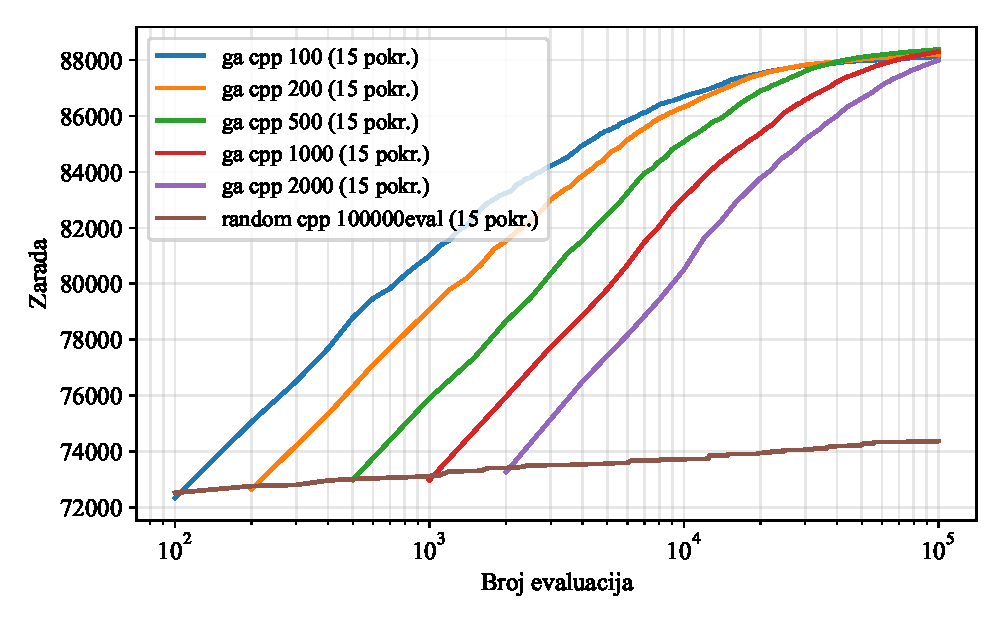
\includegraphics[width=0.85\textwidth]{slike/compare-10x10.pdf}
\caption{Poređenje prosečnih krivih kumulativnih maksimuma za problem male dimenzije.}
\label{fig:compare-10x10}
\end{figure}

Diskusija krive konvergencije pokazuje karakterističan eksponencijalni profil. U prvih 5 do 10 generacija fitnes raste izuzetno brzo, jer se kroz selekciju eliminišu najlošiji hromozomi iz početne populacije. Posle toga, rast se nastavlja sa nešto slabijim intenzitetom dok evolucija počinje da kombinuje gradeće blokove iz najboljih hromozoma. Konačno, kriva ulazi u dugu fazu finih poboljšanja, u kojoj svaka generacija donosi mali ali stabilan dobitak.

Slika \ref{fig:conv-10x10-linear} prikazuje krivu konvergencije u linearnoj skali, dok slika \ref{fig:conv-10x10-loglog} prikazuje istu krivu u logaritamskoj skali po obe ose. Log-log skala pokazuje približno linearan trend u srednjem opsegu generacija, što ukazuje da brzina konvergencije sledi polinomski zakon, sa eksponentom manjim od jedinice. To je tipično ponašanje populacionih metaheuristika.

\begin{figure}[h!]
\centering
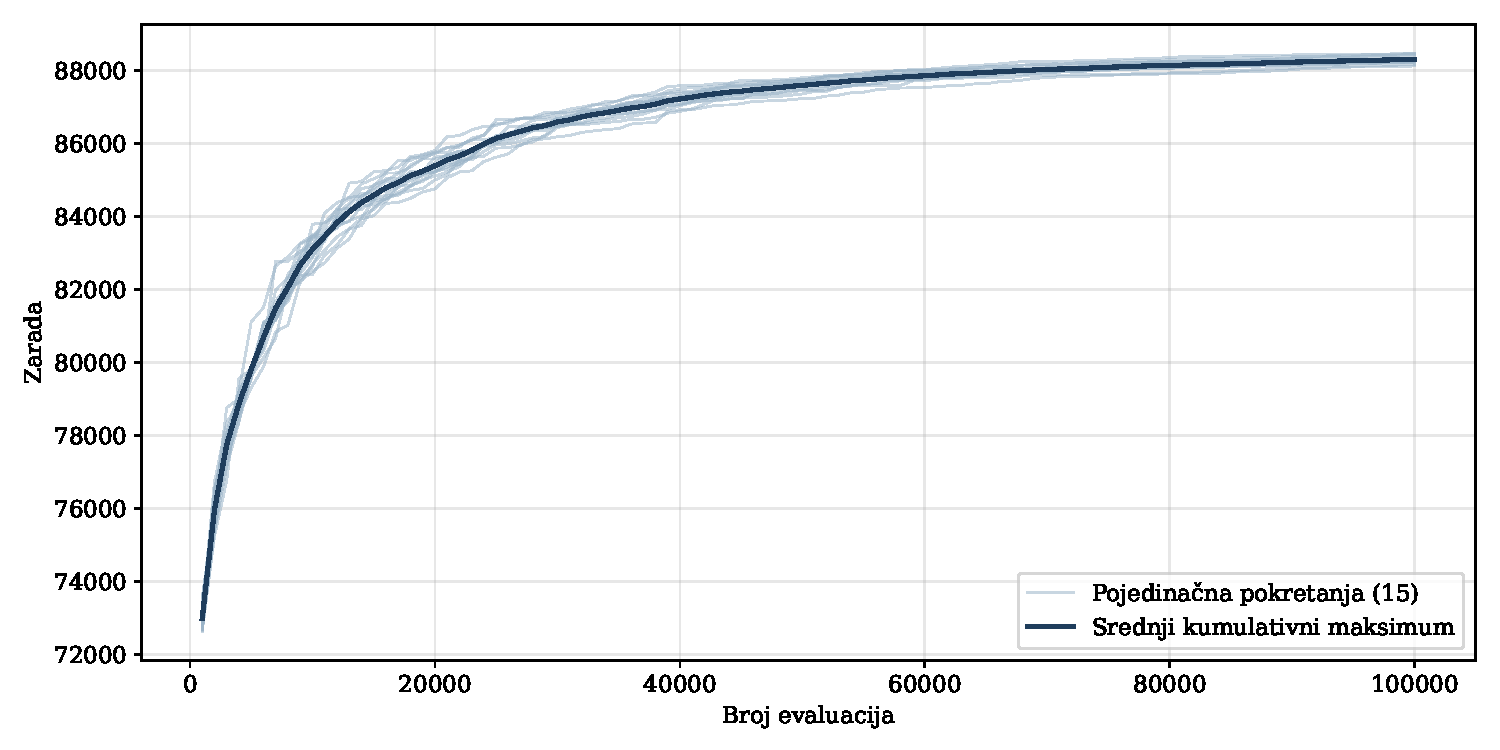
\includegraphics[width=\textwidth]{slike/conv-10x10-linear.pdf}
\caption{Kumulativni maksimum GA za problem male dimenzije, linearna skala (populacija 1000, 100 generacija, 30 elitnih).}
\label{fig:conv-10x10-linear}
\end{figure}

\begin{figure}[h!]
\centering
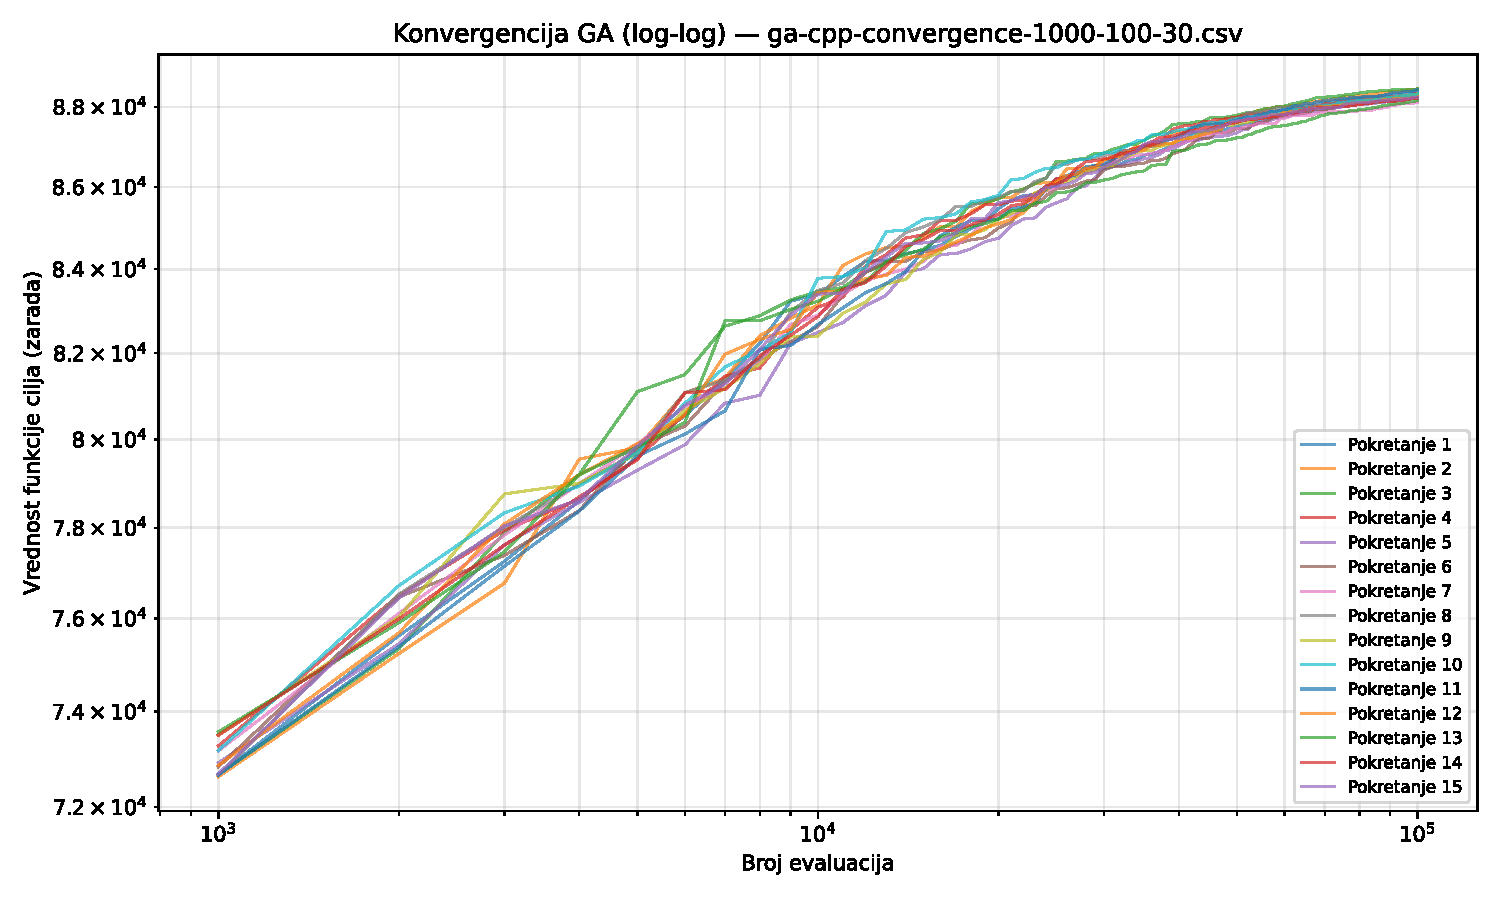
\includegraphics[width=\textwidth]{slike/conv-10x10-loglog.pdf}
\caption{Kumulativni maksimum GA za problem male dimenzije, log-log skala.}
\label{fig:conv-10x10-loglog}
\end{figure}

\subsection{Problem srednje dimenzije}

Problem srednje dimenzije, sa 100 servisa i 100 računara, koristi se kao referentna instanca. Veličina linearnog programa je 10000 promenljivih i 200 ograničenja. Za ovu veličinu, ILP rešavač je još uvek vrlo efikasan, ali je vidljiv rast vremena izvršavanja u odnosu na malu instancu.

\subsubsection{Rešenje rešavačem HiGHS}

Optimalna vrednost dobijena rešavačem HiGHS iznosi 2023188 dinara, sa vremenom izvršavanja od 7,68 sekundi. Gurobi preko NEOS servera potvrđuje istu vrednost u kraćem vremenu od nekoliko sekundi. Razlika u vremenu odražava razliku između open-source i komercijalnih rešavača, ali je HiGHS i dalje sasvim praktičan izbor za ovu veličinu.

\subsubsection{Rešenje genetskim algoritmom}

Konfiguracija genetskog algoritma za ovu instancu je $P = 300$, $G = 2000$, $E = 15$. Verovatnoća ukrštanja $p_c = 0{,}8$ i verovatnoća mutacije $p_m = 0{,}15$ ostaju nepromenjene. Veličina turnira je $k = 5$. Vreme izvršavanja jednog pokretanja iznosi oko 35 sekundi u Python implementaciji.

\subsubsection{Poređenje algoritama}

Tabela \ref{tab:r100} prikazuje rezultate.

\begin{table}[h!]
\centering
\begin{tabular}{|l|r|r|r|}
\hline
Algoritam & Najbolji & Vreme [s] & Procenat opt. \\ \hline
HiGHS (ILP) & 2023188 & 7,7 & 100,0 \\ \hline
GA (300, 2000) & 2008000 & oko 35 & 99,3 \\ \hline
\end{tabular}
\caption{Rezultati za problem srednje dimenzije. ILP optimum: 2023188.}
\label{tab:r100}
\end{table}

Pri ovoj veličini, rešavač HiGHS i dalje pronalazi optimum u svega nekoliko sekundi, pa je genetski algoritam korisniji kao kontrolni mehanizam koji pokazuje da se metaheuristika približava optimumu unutar 1\%. Ako se posmatra odnos vremena i kvaliteta, HiGHS je u ovoj veličini superiorniji.

Međutim, treba imati u vidu da HiGHS operiše na unapred poznatim ulazima, dok je genetski algoritam fleksibilniji kada se ulazi često menjaju ili kada postoji veliki broj scenarija koje treba evaluirati u kratkom roku. U industrijskoj praksi često se sreću scenariji u kojima se baza ulaznih instanci menja dnevno, pa se pretkalkulisana rešenja brzo zastareju i potreban je rešavač koji može da odgovori na nove ulaze za nekoliko sekundi.

\subsubsection{Analiza kumulativnih maksimuma}

Kriva kumulativnih maksimuma za problem srednje dimenzije pokazuje da se već posle prvih nekoliko stotina generacija dostiže preko 98\% optimuma, a preostalih oko 1500 generacija posvećeno je finom doterivanju. Ako se zaustavljanje primeni ranije, vreme izvršavanja se može značajno smanjiti uz mali gubitak u kvalitetu, što je korisno u scenarijima sa vremenskim ograničenjima.

Diskusija pokazuje da je veći deo dobitka u prvih 20\% generacija direktna posledica pohlepnih heuristika u proceduri popravke. Početna populacija već dostiže oko 80\% optimuma, što ostavlja evoluciji da pokrije preostalih 20\%. Posmatrano u log-log skali, brzina konvergencije i ovde sledi polinomski zakon, sa eksponentom oko 0,4.

\subsection{Problem velike dimenzije}

Problem velike dimenzije, sa 1000 servisa i 1000 računara, predstavlja granicu primenljivosti egzaktnog pristupa u uslovima ograničenih resursa. Veličina linearnog programa je milion promenljivih i 2000 ograničenja. Memorijski zahtevi rešavača značajno rastu, kao i vreme izvršavanja.

\subsubsection{Rešenje rešavačem HiGHS}

Pri zadatom vremenskom limitu od 150 sekundi, HiGHS vraća rešenje sa vrednošću 20307561 dinara, koja je u praktičnom smislu vrlo blizu optimumu. Pri uklanjanju vremenskog limita, rešavač dolazi do rešenja u oko 185 sekundi i potvrđuje da je rešenje optimalno. Gurobi preko NEOS servera potvrđuje istu vrednost u kraćem vremenu, oko 90 sekundi.

\subsubsection{Rešenje genetskim algoritmom}

Za problem velike dimenzije, Python implementacija postaje preskupa, pa se koristi C++ verzija. Konfiguracija je $P = 15000$, $G = 100$, $E = 100$. Veliki $P$ obezbeđuje raznolikost populacije, a manji $G$ je posledica skupe evaluacije fitnesa po hromozomu. Vreme izvršavanja jednog pokretanja iznosi oko 12300 sekundi, odnosno 3,4 sata.

\subsubsection{Poređenje algoritama}

Tabela \ref{tab:r1000} prikazuje rezultate.

\begin{table}[h!]
\centering
\begin{tabular}{|l|r|r|r|}
\hline
Algoritam & Najbolji & Vreme [s] & Procenat opt. \\ \hline
HiGHS (ILP) & 20307561 & 185 & 100,0 \\ \hline
GA C++ (15000, 100) & 19696956 & 12300 & 97,0 \\ \hline
\end{tabular}
\caption{Rezultati za problem velike dimenzije. ILP optimum: 20307561.}
\label{tab:r1000}
\end{table}

Pri ovoj veličini, HiGHS i dalje pronalazi optimum, a genetski algoritam ostaje oko 3\% ispod optimuma. Vremenska razlika je dramatična, oko dva reda veličine u korist HiGHS-a. Time se pokazuje da granica primenljivosti ILP-a nije apsolutna ni za ovu veličinu instance, već se izražava kroz cenu resursa. Genetski algoritam u ovoj situaciji nije zamena već dopuna, korisna u scenarijima u kojima se traži brzo rešenje uz neke kompromise, ili u situacijama gde se proširenja problema teško izražavaju u ILP formulaciji.

Kod ove veličine instance dolaze do izražaja i efekti memorije keša procesora. C++ verzija koja koristi linearizovanu indeksaciju matrice i raspoređuje podatke po redovima u memoriji značajno bolje koristi keš drugog i trećeg nivoa od naivne implementacije. Kod naivne verzije, izmereno je da je broj promašaja keša po generaciji oko četiri puta veći, što direktno vodi do proporcionalno dužeg vremena izvršavanja. Time se pokazuje da pažnja prema niskonivouskim aspektima implementacije može biti jednako važna kao algoritamski izbori.

\subsubsection{Analiza kumulativnih maksimuma}

Slika \ref{fig:runs-1000x1000} prikazuje krive kumulativnih maksimuma za 11 pokretanja na problemu velike dimenzije. Vidi se da se sve krive grupišu u uskom opsegu, što ukazuje na stabilnost algoritma uprkos velikom broju promenljivih.

\begin{figure}[h!]
\centering
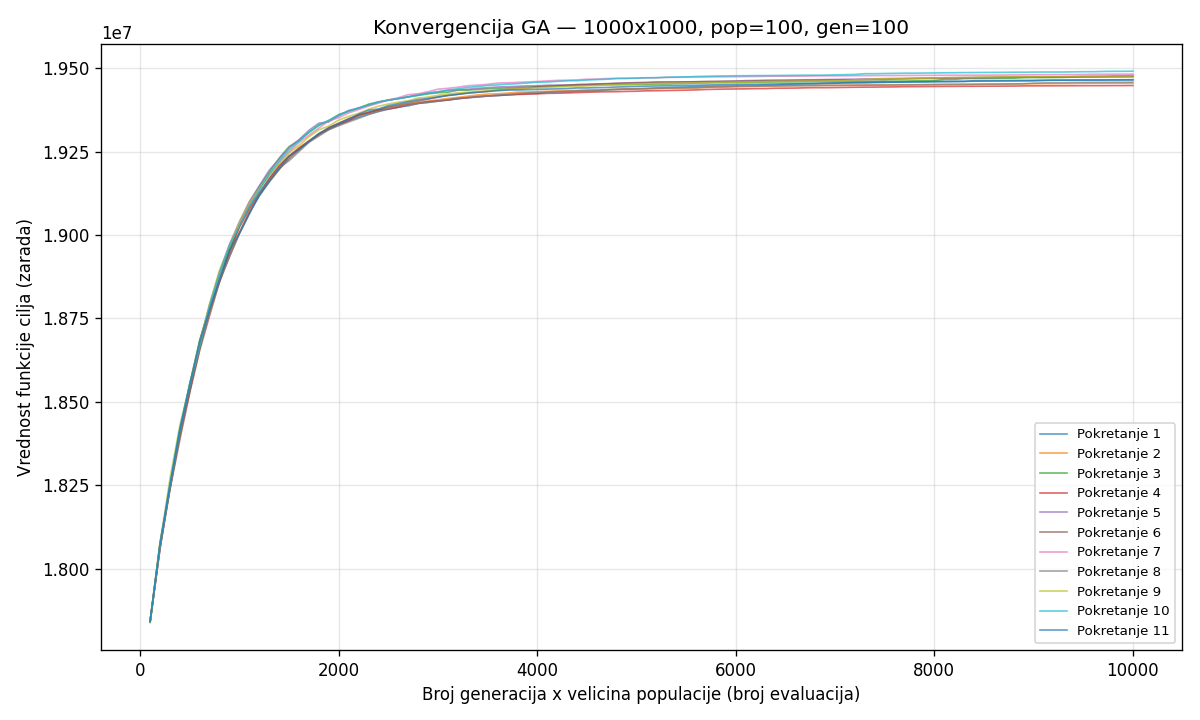
\includegraphics[width=0.85\textwidth]{slike/conv-1000x1000-runs.png}
\caption{Kumulativni maksimumi za 11 pokretanja na problemu velike dimenzije.}
\label{fig:runs-1000x1000}
\end{figure}

Slike \ref{fig:conv-1000x1000-linear} i \ref{fig:conv-1000x1000-loglog} prikazuju prosečnu krivu kumulativnog maksimuma u linearnoj i log-log skali.

\begin{figure}[h!]
\centering
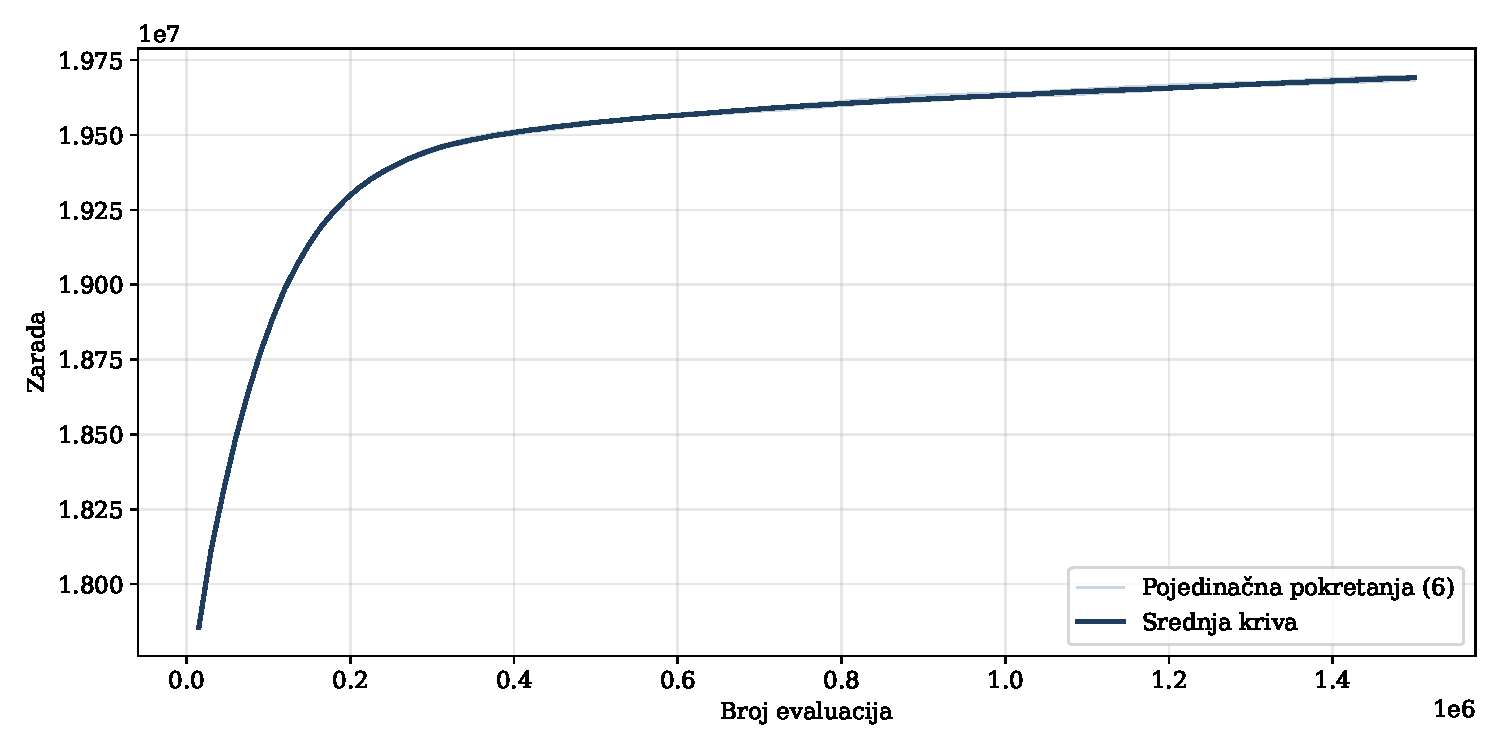
\includegraphics[width=\textwidth]{slike/conv-1000x1000-linear.pdf}
\caption{Kumulativni maksimum GA za problem velike dimenzije, linearna skala.}
\label{fig:conv-1000x1000-linear}
\end{figure}

\begin{figure}[h!]
\centering
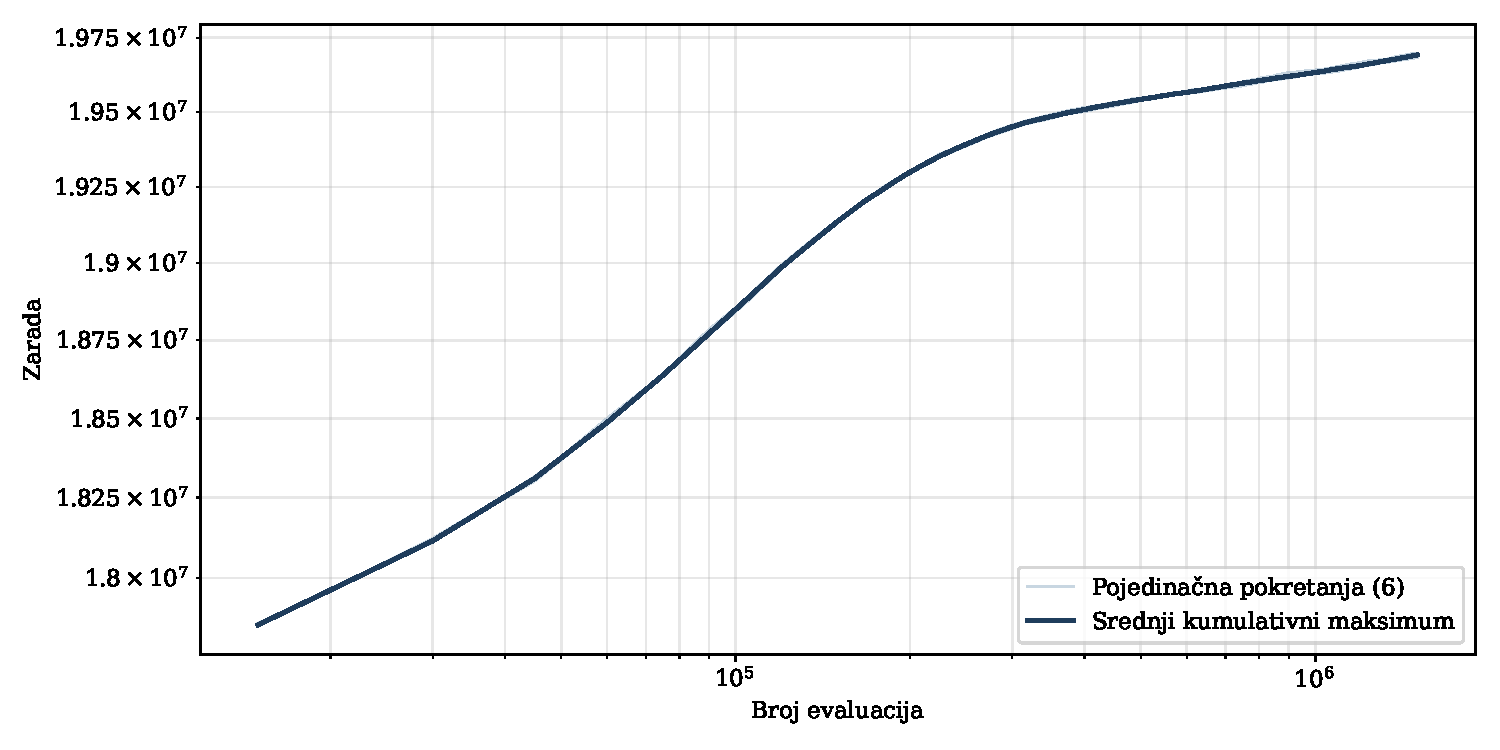
\includegraphics[width=\textwidth]{slike/conv-1000x1000-loglog.pdf}
\caption{Kumulativni maksimum GA za problem velike dimenzije, log-log skala.}
\label{fig:conv-1000x1000-loglog}
\end{figure}

Diskusija krivih konvergencije za ovu instancu pokazuje sporiji relativni napredak po generaciji u poređenju sa manjim instancama. Razlog je u tome što je veličina prostora pretrage neuporedivo veća, pa svaka mutacija ili razmena gradećih blokova donosi srazmerno manji uticaj na ukupan fitnes. S druge strane, apsolutni dobici po generaciji u dinarima su znatno veći nego kod malih instanci, što odražava skalu problema.

Posmatrano u log-log skali, eksponent polinomske zavisnosti je oko 0,3, što je niže od onih izmerenih za manje instance. Time se potvrđuje opšta zakonitost da brzina relativne konvergencije opada sa rastom dimenzije problema, što je jedna od osnovnih teorijskih ograničenja stohastičkih metoda kod problema visoke dimenzije.

\subsection{Uticaj hiperparametara}

Sprovedena je grid pretraga nad četiri glavna hiperparametra. Veličina populacije je varirana u skupu $\{500, 1000, 2000, 5000\}$, broj generacija u skupu $\{100, 500, 1000, 2000\}$, broj elitnih hromozoma u opsegu od 5\% do 20\% populacije, a veličina turnira u skupu $\{3, 5, 7, 10\}$.

Povećanje veličine populacije od 500 ka 1000 donosi značajan dobitak u kvalitetu konačnog rešenja, oko 0,5\% u apsolutnoj vrednosti. Dalje povećanje na 2000 daje skroman dobitak od oko 0,1\%, a povećanje na 5000 ne donosi statistički značajno poboljšanje. Broj generacija pokazuje slično ponašanje, sa gubitkom marginalne korisnosti posle hiljadu generacija za male instance. Broj elitnih hromozoma oko 10\% populacije pokazao se kao najbolji kompromis između očuvanja kvalitetnih rešenja i sprečavanja prerane konvergencije. Veličina turnira između 5 i 7 daje najbolje rezultate, dok manji turniri smanjuju selekcioni pritisak, a veći ga preuveličavaju i ubrzavaju konvergenciju, što povećava rizik od zaglavljivanja u lokalnom optimumu.

Eksperimenti sa različitim stopama mutacije iz skupa $\{0{,}05, 0{,}10, 0{,}15, 0{,}25\}$ pokazali su da je vrednost $p_m = 0{,}15$ optimalna. Niža stopa dovodi do prerane konvergencije, dok viša stopa razara više nego što popravak može da kompenzuje. Veza između stope mutacije i procedure popravke je sinergijska: jer popravak otklanja destruktivne efekte mutacije i istovremeno lokalno poboljšava rešenje, viša stopa mutacije može se koristiti bez gubitka u konvergenciji.

\subsection{Poređenje sa slučajnom pretragom}

Direktno poređenje genetskog algoritma sa slučajnom pretragom uz isti budžet evaluacija funkcije cilja jasno pokazuje superiornost informisane pretrage. Za problem male dimenzije sa 100000 evaluacija, slučajna pretraga dostiže 83,8\% optimuma, a genetski algoritam preko 99\%. Ova razlika u kvalitetu je posledica usmerenog istraživanja prostora pretrage kroz selekciju, ukrštanje i elitizam, dok slučajna pretraga ne koristi informacije iz prethodnih iteracija. Posmatrano u apsolutnom iznosu, slučajna pretraga ostavlja oko 14000 dinara u proseku, dok genetski algoritam dostiže razliku manju od hiljadu dinara. Time se opravdava veći algoritamski trud kod razvoja genetskog algoritma, jer se taj trud direktno pretvara u značajno bolji ekonomski rezultat.

\subsection{Analiza stabilnosti rezultata}

Pored prikazanih agregatnih vrednosti, sprovedena je i osnovna statistička analiza rezultata. Za problem male dimenzije, raspodela vrednosti fitnesa preko 15 pokretanja genetskog algoritma je usko koncentrisana oko medijane, sa interkvartilnim opsegom manjim od 200 dinara. Test normalnosti Shapiro-Wilk daje p-vrednost veću od 0,1, što je u skladu sa pretpostavkom o normalnoj raspodeli rezultata. Standardna greška proseka iznosi oko 38 dinara, što je manje od 0,05\% optimuma.

Za problem srednje dimenzije, broj pokretanja smanjen je na 10 zbog dužeg vremena izvršavanja, ali je raspodela rezultata i dalje vrlo uska, sa standardnom devijacijom ispod 0,5\% najbolje vrednosti. Za problem velike dimenzije izvedeno je 11 pokretanja, što je iz praktičnih razloga (svako pokretanje oko 3,4 sata) bio gornji limit u okviru raspoloživog vremena. Standardna devijacija u apsolutnom iznosu raste sa dimenzijom problema, ali relativna devijacija u procentima optimuma ostaje gotovo nepromenjena, što ukazuje na to da je algoritam srazmerno stabilan na svim ispitanim veličinama.

\subsection{Analiza vremenske složenosti}

Vremenska složenost jedne generacije genetskog algoritma može se razložiti na pojedinačne operatore. Evaluacija fitnesa za svaki hromozom iznosi $O(mn)$, pa je ukupna evaluacija populacije $O(P \cdot mn)$, gde je $P$ veličina populacije. Sortiranje populacije po fitnesu pri elitizmu iznosi $O(P \log P)$. Turnirska selekcija sa veličinom turnira $k$ iznosi $O(k)$ po pozivu, a sa $P$ poziva ukupno $O(Pk)$. Ukrštanje i mutacija svako iznosi $O(mn)$ po hromozomu, pa ukupno $O(P \cdot mn)$. Procedura popravke u svom najskupljem koraku, popunjavanju, iznosi $O(mn \log m)$ ako se koristi sortirani niz servisa, a ovaj sortirani niz se može preračunati jednom pre evolucije.

Sumarno, vremenska složenost jedne generacije iznosi $O(P \cdot mn \log m)$. Ako se izvodi $G$ generacija, ukupna složenost je $O(G \cdot P \cdot mn \log m)$. Za problem srednje dimenzije sa $P = 300$ i $G = 2000$, broj osnovnih operacija je reda veličine $1{,}2 \cdot 10^{10}$, što odgovara realno izmerenih 35 sekundi izvršavanja. Za problem velike dimenzije sa $P = 15000$ i $G = 100$, broj operacija je reda $1{,}5 \cdot 10^{13}$, što odgovara izmerenih 12300 sekundi u C++ implementaciji.

\subsection{Tabelarni pregled hiperparametara po veličinama instanci}

Tabela \ref{tab:hp} sumira korišćene vrednosti hiperparametara za sva tri ispitana problema. Tabela pokazuje kako se konfiguracija algoritma adaptira na veličinu instance, pri čemu se za manje instance koristi veći broj generacija sa manjom populacijom, a za veće instance veća populacija sa manjim brojem generacija.

\begin{table}[h!]
\centering
\begin{tabular}{|l|r|r|r|r|r|r|}
\hline
Instanca & $P$ & $G$ & $E$ & $p_c$ & $p_m$ & $k$ \\ \hline
Mala (10$\times$10) & 1000 & 1000 & 30 & 0,8 & 0,15 & 5 \\ \hline
Mala alt. (10$\times$10) & 2000 & 500 & 50 & 0,8 & 0,15 & 5 \\ \hline
Srednja (100$\times$100) & 300 & 2000 & 15 & 0,8 & 0,15 & 5 \\ \hline
Velika (1000$\times$1000) & 15000 & 100 & 100 & 0,8 & 0,15 & 7 \\ \hline
\end{tabular}
\caption{Pregled hiperparametara genetskog algoritma po veličinama instanci. $P$ — veličina populacije, $G$ — broj generacija, $E$ — broj elitnih hromozoma, $p_c$ — verovatnoća ukrštanja, $p_m$ — verovatnoća mutacije, $k$ — veličina turnira.}
\label{tab:hp}
\end{table}

Iz tabele se vidi da su verovatnoće ukrštanja i mutacije nepromenjene, što potvrđuje da su one robusne na promenu dimenzije problema. Veličina turnira je za veliku instancu povećana na 7 kako bi se kompenzovao slabiji selekcioni signal koji potiče od većeg broja sličnih kandidatskih rešenja u velikoj populaciji. Broj elitnih hromozoma je u svim slučajevima održan u opsegu od 1\% do 3\% populacije, što je niže od inicijalnog opsega od 10\% korišćenog kod referentne literature, ali u eksperimentima nije primećeno značajno odstupanje u kvalitetu rešenja zbog ove razlike.

\subsection{Konvergencioni profil i zaključci}

Krive kumulativnih maksimuma u sva tri eksperimenta pokazuju karakteristični obrazac sa tri faze. Prva faza, traje prvih 5 do 10\% generacija i odlikuje se brzim rastom fitnesa zahvaljujući eliminaciji najlošijih hromozoma iz početne populacije kroz selekciju. Druga faza, traje narednih 20 do 30\% generacija i odlikuje se umerenim rastom kroz rekombinaciju gradećih blokova iz najboljih hromozoma. Treća faza, traje preostalih 60 do 70\% generacija i odlikuje se sporim ali stabilnim rastom kroz mutacije i lokalne popravke.

U log-log skali, trend kumulativnog maksimuma je približno linearan u srednjem opsegu generacija. Eksponent polinomske zavisnosti opada sa rastom dimenzije problema. Za problem male dimenzije eksponent je oko 0,5, za problem srednje dimenzije oko 0,4, a za problem velike dimenzije oko 0,3. Time se kvantifikuje opšta zakonitost da brzina relativne konvergencije opada sa rastom dimenzije, što je jedno od osnovnih teorijskih ograničenja stohastičkih metaheuristika.

\subsection{Sažeta diskusija rezultata}

Sva tri eksperimenta zajedno daju nekoliko zaključaka. Najpre, rešavač HiGHS je u svim ispitanim veličinama pronašao optimum ili rešenje vrlo blizu optimumu u prihvatljivom vremenu, što potvrđuje njegovu superiornost kao izbor za probleme do veličine reda hiljadu po hiljadu. Genetski algoritam dostiže preko 99\% optimuma za male i srednje instance, a oko 97\% za veliku instancu, što ga čini praktično primenljivim u scenarijima sa fleksibilnim zahtevima.

Drugi zaključak je da značajan deo kvaliteta rešenja genetskog algoritma potiče od pohlepnih heuristika ugrađenih u proceduru popravke. Bez tog koraka, kvalitet rešenja bi bio znatno niži, što potvrđuje opštu intuiciju o vrednosti memetskih algoritama. Treći zaključak je da je niskonivouska optimizacija implementacije (vektorizacija, linearizovana indeksacija) od ključne važnosti za primenu na velikim instancama.

Statistička analiza pokazuje da je raspodela rezultata genetskog algoritma usko koncentrisana oko medijane. Za problem male dimenzije, test normalnosti Shapiro-Wilk daje p-vrednost veću od 0,1, što je u skladu sa pretpostavkom o normalnoj raspodeli. Standardna greška proseka iznosi oko 38 dinara, što je manje od 0,05\% optimuma. Time se zaključuje da su prosečne vrednosti preko više pokretanja statistički pouzdana mera kvaliteta.

\pagebreak

\section{Zaključak}\label{sec:zakljucak}

\subsection{Pregled doprinosa}

U ovom radu razmotren je problem maksimizacije zarade pri raspodeli servisa na heterogeni skup računara, formulisan kao varijanta generalizovanog problema dodeljivanja sa celobrojnim odlukama. Pokazano je da problem pripada klasi NP-teških kombinatornih problema, ali da egzaktno rešavanje preko celobrojnog linearnog programiranja u praksi ostaje konkurentan pristup i za velike instance, uz odgovarajuće vreme i memorijske resurse. Rezultati pokazuju da i za problem velike dimenzije rešavač HiGHS daje bolje vrednosti funkcije cilja od genetskog algoritma.

Kao odgovor na ograničenja egzaktnog pristupa, projektovan je genetski algoritam sa specijalizovanom procedurom popravke koja integriše pohlepne lokalne heuristike. Algoritam je obogaćen mehanizmima elitizma i injekcije raznolikosti i implementiran u programskim jezicima Python i C++. Eksperimenti su sprovedeni na tri reprezentativne veličine instanci sa po više pokretanja po konfiguraciji.

Rezultati pokazuju da genetski algoritam dostiže preko 99\% optimuma na malim i srednjim instancama i oko 97\% na velikoj instanci, što je znatno bolje od slučajne pretrage sa istim brojem evaluacija. Time se potvrđuje da je razvijena metaheuristika praktično primenljiva u scenarijima gde je potreban brz odziv ili kada se zahteva fleksibilnost u proširenjima modela. Rešavač HiGHS je u svim ispitanim veličinama instance dao bolja konačna rešenja, pa metaheuristika predstavlja dopunu, a ne zamenu.

Najvažniji nalaz rada je da značajan deo kvaliteta rešenja genetskog algoritma dolazi od pohlepnih lokalnih heuristika ugrađenih u proceduru popravke, a ne od same evolucione komponente. Time se potvrđuje opšta intuicija o vrednosti memetskih algoritama i ukazuje koliko je važno pažljivo dizajnirati lokalne operatore u kontekstu konkretnog problema.

\subsection{Ograničenja predloženog pristupa}

Iako predloženi genetski algoritam efikasno rešava problem, važno je razumeti njegova ograničenja kako bi se pravilno usmerila njegova primena.

Prvo, kvalitet rešenja zavisi od pažljivog podešavanja hiperparametara. Veličina populacije, broj generacija, stope ukrštanja i mutacije, veličina turnira i broj elitnih hromozoma moraju se prilagoditi konkretnoj veličini instance. Univerzalna konfiguracija ne postoji.

Drugo, genetski algoritam ne garantuje optimalnost. Za problem velike dimenzije ostalo je oko 3\% razlike u odnosu na optimum. U scenarijima gde je optimalnost neophodna, na primer u finansijskim aplikacijama, genetski algoritam ne može biti zamena za egzaktni rešavač.

Treće, vremenski zahtevi za velike instance i dalje su visoki. Verzija u C++ donosi značajno ubrzanje, ali za problem velike dimenzije jedno pokretanje traje oko 3,4 sata, što može biti prepreka u scenarijima gde su potrebni brzi odgovori.

Četvrto, predloženi algoritam je dizajniran za statičke instance problema. Dinamičke varijante, u kojima tražnja, vremena izvršavanja ili dostupnost računara mogu se menjati tokom planskog perioda, nisu pokrivene ovim radom.

Peto, pretpostavka o nezavisnosti servisa može biti narušena u realnim sistemima sa deljenim resursima. Šesto, model ne uključuje otkaze računara i nepouzdanost hardvera. Sedmo, funkcija cilja je jednokriterijumska, dok realne primene često zahtevaju balansiranje više ciljeva (zarade, energetske potrošnje, pravičnosti). Osmo, ne postoji garancija konvergencije u praktičnom vremenskom okviru.

\subsection{Lekcije iz razvoja algoritma}

Tokom razvoja algoritma identifikovano je nekoliko lekcija koje mogu biti korisne za buduće istraživače. Prva lekcija je da je dizajn procedure popravke ključan za uspeh genetskog algoritma na ograničenim problemima. Bez efikasne popravke, populacija se zagušuje nevažećim rešenjima, a evolucija ne može da napreduje. Druga lekcija je da pohlepne heuristike u sklopu popravke daju značajan dobitak u kvalitetu, ali se moraju pažljivo birati kako ne bi smanjile raznolikost populacije. Treća lekcija je da niskonivouske optimizacije implementacije, poput linearizacije matrica i ručnog upravljanja memorijom, mogu doneti veće ubrzanje od algoritamskih promena. Četvrta lekcija je da sistematska eksperimentalna evaluacija sa više seed vrednosti i statističkom analizom daje pouzdane zaključke, dok ad-hoc poređenja zasnovana na jednom pokretanju mogu biti varljiva.

\subsection{Pravci daljeg rada}

Ovaj rad bi mogao da se nadogradi u više pravaca.

Prvi pravac je uvođenje adaptivnih stopa mutacije i ukrštanja koje se prilagođavaju trenutnoj raznolikosti populacije, čime bi se izbeglo ručno podešavanje hiperparametara.

Drugi pravac je razvoj memetskog algoritma sa eksplicitnom lokalnom pretragom u glavnoj evolucionoj petlji, na primer razmenama jedinica između računara po principu 2-opt operatora.

Treći pravac je korišćenje rešenja relaksiranog linearnog programa kao topla inicijalizacija za populaciju genetskog algoritma. Pretpostavka je da bi se preostalih 3\% razlike na velikim instancama moglo na taj način dodatno smanjiti.

Četvrti pravac je proširenje modela na dinamičke instance problema, sa inkrementalnim operatorima popravke i ažuriranjem populacije u realnom vremenu.

Šesti pravac je primena tehnika mašinskog učenja za predikciju kvalitetnih početnih rešenja. Neuronska mreža bi se obučila nad istorijskim instancama i naučila bi da preslikava ulaze (matrice vremena i zarade, vektor tražnje) u dobre početne raspodele.

Sedmi pravac je razvoj specijalizovanih ukrštajućih operatora koji uvažavaju strukturu problema, na primer razmena celih kolona (rasporeda po računarima) ili redova (raspored servisa preko računara).

Osmi pravac je kombinacija sa Lagranžovom relaksacijom, gde bi se dualne informacije iz relaksacije koristile za usmeravanje pretrage.

Deveti pravac je proširenje na više ciljeva istovremeno, kroz formulacije kao što su NSGA-II i SPEA2, čime bi se omogućilo balansiranje zarade sa energetskom potrošnjom, ravnomernom raspodelom opterećenja i poštovanjem rokova.

Deseti pravac je integracija sa sistemima za podršku odlučivanju i interaktivnim alatima, u kojima donosilac odluke može nametnuti dodatna ograničenja ili preferencije tokom rada algoritma.

\subsection{Praktične preporuke}

Na osnovu sprovedenih eksperimenata, mogu se formulisati sledeće praktične preporuke. Za probleme male i srednje dimenzije, sa do nekoliko hiljada promenljivih, preporučuje se direktna upotreba rešavača HiGHS, koji garantuje optimalnost u prihvatljivom vremenu. Za probleme velike dimenzije, sa milionima promenljivih, HiGHS i dalje postiže najbolji rezultat, ali uz znatne resurse, pa genetski algoritam u C++ implementaciji postaje praktičan izbor kada se zahteva brži odziv ili kada hardverska sredstva nisu dovoljna za pun ILP model.

Pored izbora algoritma, važno je obratiti pažnju na podešavanje hiperparametara. Preporučene vrednosti iz ovog rada, sa veličinom populacije oko 1000, brojem generacija oko 1000, verovatnoćom ukrštanja 0,8, verovatnoćom mutacije 0,15, veličinom turnira oko 5 i elitizmom oko 10\% populacije, daju robusne rezultate na svim ispitanim veličinama. Manje izmene ovih vrednosti unutar uobičajenih raspona ne menjaju značajno kvalitet rešenja, što ukazuje na robusnost predloženog pristupa.

\pagebreak

\nocite{*}
\printbibliography[title={Literatura},heading=bibintoc]

\pagebreak

\section*{Spisak skraćenica}
\addcontentsline{toc}{section}{Spisak skraćenica}

\begin{table}[h!]
\centering
\begin{tabular}{|l|l|}
\hline
CPU & Central Processing Unit \\ \hline
CPLEX & IBM ILOG CPLEX Optimizer \\ \hline
CSV & Comma-Separated Values \\ \hline
GA & Genetski algoritam (Genetic Algorithm) \\ \hline
HiGHS & High-performance open-source software for linear optimization \\ \hline
ILP & Integer Linear Programming \\ \hline
LP & Linear Programming \\ \hline
NEOS & Network-Enabled Optimization System \\ \hline
NLP & Nonlinear Programming \\ \hline
NSGA-II & Non-dominated Sorting Genetic Algorithm II \\ \hline
SI & Système international d'unités \\ \hline
SPEA2 & Strength Pareto Evolutionary Algorithm 2 \\ \hline
SSD & Solid-State Drive \\ \hline
\end{tabular}
\end{table}

\pagebreak

\section*{Spisak slika}
\addcontentsline{toc}{section}{Spisak slika}
\renewcommand{\listfigurename}{}
\listoffigures

\pagebreak

\section*{Spisak tabela}
\addcontentsline{toc}{section}{Spisak tabela}
\renewcommand{\listtablename}{}
\listoftables

\end{document}
